\begin{tikzpicture}
	%\draw[help lines] (0,0) grid (6,4);
	\begin{axis}[axis lines=middle, axis equal, grid=both, xlabel = $\operatorname{Re}$, ylabel = $\operatorname{Im}$]
		\draw (axis cs: 0, 0) circle [black!10, radius=1];
		\addplot[patch, opacity=0.5, table/row sep=\\, patch table={%
			0 1 2\\
			1 2 3\\
			4 3 5\\
		}]
		table[row sep=\\,point meta=\thisrow{c}] {
			x		y		c	\\
			1		0 		1	\\% 0
			0		0		1	\\% 2
			0.31	0.95	0.5	\\% 1
			-0.81	0.59	1	\\% 3
			0		0		0.5	\\% 2
			-0.81	0		1	\\% 4
		};
		\addplot[patch, opacity=0.5, table/row sep=\\, patch table={%
			0 1 2\\
			1 2 3\\
			4 3 5\\
		}]
		table[row sep=\\,point meta=\thisrow{c}] {
			x		y		c	\\
			1		0 		1	\\% 0
			0		0		1	\\% 2
			0.31	-0.95	0.5	\\% 1
			-0.81	-0.59	1	\\% 3
			0		0		0.5	\\% 2
			-0.81	0		1	\\% 4
		};
		\draw[latex-latex, red]  ([shift=(60:1cm)]90, 84) arc(0:55:1cm) node[midway, rotate=30, right, red] {$\varphi = \dfrac{2\pi}{5}$};
		\addplot[orange, very thick, mark=*] coordinates{(1, 0) (1, 0)} node[above, red!70] {$e_1^{(5)}$};
		\addplot[orange, very thick, mark=*] coordinates{(0.31, 0.95) (0.31, 0.95)} node[above, red!70, right] {$e_2^{(5)}$};
		\addplot[orange, very thick, mark=*] coordinates{(-0.81, 0.59) (-0.81, 0.59)} node[above, red!70] {$e_3^{(5)}$};
		\addplot[orange, very thick, mark=*] coordinates{(-0.81, -0.59) (-0.81, -0.59)} node[above, red!70] {$e_4^{(5)}$};
		\addplot[orange, very thick, mark=*] coordinates{(0.31, -0.95) (0.31, -0.951)} node[above, red!70, right] {$e_5^{(5)}$};
		\addplot[->, dashed, white] coordinates{(0.8, 1.1) (0.8, 1.2)}; % for axis-scaling
		\addplot[->, dashed, white] coordinates{(0.8, -1) (0.8, -1.2)}; % for axis-scaling
	\end{axis}
\end{tikzpicture}